\documentclass[a4paper]{article}

%use the english line for english reports
%usepackage[english]{babel}
\usepackage[portuguese]{babel}
\usepackage[utf8]{inputenc}
\usepackage{indentfirst}
\usepackage{graphicx}
\usepackage{verbatim}
\usepackage{listings}
\usepackage{float}
\usepackage{wrapfig}

\begin{document}

\setlength{\textwidth}{16cm}
\setlength{\textheight}{22cm}

\title{\Huge\textbf{Oolong}\linebreak\linebreak\linebreak
\Large\textbf{Relatório Intercalar}\linebreak\linebreak
\linebreak\linebreak

\includegraphics[scale=0.1]{feup-logo.png}\linebreak\linebreak
\linebreak\linebreak
\Large{Mestrado Integrado em Engenharia Informática e Computação} \linebreak\linebreak
\Large{Programação em Lógica}\linebreak
}

\author{\textbf{Grupo Oolong\_1:}\\
José Pedro Borges - up201503603 \\
Miguel Mano Fernandes - up201503538 \\
\linebreak\linebreak \\
 \\ Faculdade de Engenharia da Universidade do Porto \\ Rua Roberto Frias, s\/n, 4200-465 Porto, Portugal \linebreak\linebreak\linebreak
\linebreak\linebreak\vspace{1cm}}

\maketitle
\thispagestyle{empty}

%************************************************************************************************
%************************************************************************************************

\newpage

%Todas as figuras devem ser referidas no texto. %\ref{fig:codigoFigura}
%
%%Exemplo de código para inserção de figuras
%%\begin{figure}[h!]
%%\begin{center}
%%escolher entre uma das seguintes três linhas:
%%\includegraphics[height=20cm,width=15cm]{path relativo da imagem}
%%\includegraphics[scale=0.5]{path relativo da imagem}
%%\includegraphics{path relativo da imagem}
%%\caption{legenda da figura}
%%\label{fig:codigoFigura}
%%\end{center}
%%\end{figure}
%
%
%\textit{Para escrever em itálico}
%\textbf{Para escrever em negrito}
%Para escrever em letra normal
%``Para escrever texto entre aspas''
%
%Para fazer parágrafo, deixar uma linha em branco.
%
%Como fazer bullet points:
%\begin{itemize}
	%\item Item1
	%\item Item2
%\end{itemize}
%
%Como enumerar itens:
%\begin{enumerate}
	%\item Item 1
	%\item Item 2
%\end{enumerate}
%
%\begin{quote}``Isto é uma citação''\end{quote}


%%%%%%%%%%%%%%%%%%%%%%%%%%
\section{O Jogo Oolong}

Oolong é um jogo de tabuleiro desenvolvido em 2015 pelo artista John Shulters e designer Sarah Graybill, publicado por Black Straw Games. \newline


Trata-se de um jogo de estratégia para dois jogadores situado numa casa de chá japonesa, em que cada jogador representa um fabricante de chá (preto e verde) tentando servir o máximo da sua marca. 

Quando um jogador servir 5 porções numa mesa, haverá atingido a maioria nessa mesa. Vencer o jogo envolve atingir a maioria em 5 mesas e, consequentemente, na casa. \newline

A organização das 9 mesas deverá seguir a seguinte estrutura: \newline
\begin{center}
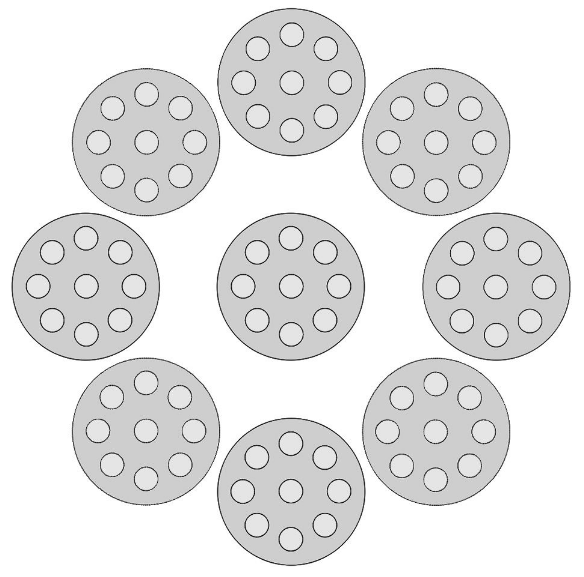
\includegraphics[scale=0.5]{board-setup.png}\newline
\end{center}

Como cada uma das 9 mesas tem 9 posições para jogar será mais fácil imaginar uma bússola por cima do tabuleiro em que cada lugar na mesa e cada mesa representam uma direção (N, NE, E, SE, S, (...) e centro). 

\subsection{Regras do Jogo}
\subsubsection{Começar o jogo}
Quem começa o jogo é o jogador com o chá preto e tem de colocar uma das peças dele na mesa do centro, em qualquer posição. Se os jogadores estiverem envolvidos em múltiplos jogos, quem começa é quem perdeu o último. 

Cada jogada envolve colocar uma peça, mover o empregado e, possivelmente, ativar uma Ação Especial.

\subsubsection{Colocação de peças}
O lugar em que a peça é colocada indica a mesa em que se vai jogar a seguir. Por exemplo, se o jogador Verde jogar no lugar SE da mesa do centro, o jogador Preto tem de jogar na mesa SE do tabuleiro, em qualquer posição, desde que não esteja já ocupada.

\newpage
\subsubsection{Mover o empregado}
O empregado é utilizado para ajudar a saber em que mesa será colocada a próxima peça e a sua posição prévia. As regras de utilização são as seguintes:
\begin{itemize}
\item Quando é jogada uma peça, o empregado é movido para a mesa onde vai ser feita a próxima jogada.
\item Ao colocar o empregado é preciso ter o cuidado de o pôr na peça que represente a mesa onde foi jogado o turno anterior.
\end{itemize}

Por exemplo, se o jogador Preto está na mesa do centro e joga na posição W, é preciso colocar o empregado na mesa W e na posição do centro desta.

\subsection{Marcadores especiais}

Existem 8 marcadores especiais que são designados aleatoriamente às mesas na periferia - cada mesa tem um no máximo. 

Cada marcador é ativado imediatamente mal o requisito que exigido seja cumprido. Após a ação ter sido feita não poderá voltar a ser usado até ao final do jogo. Se uma ação ativar outra ação noutra mesa, esta também será executada, ou seja, é permitido encadeamento de ações especiais. \newline

Eis os 5 tipos principais de marcadores presentes numa partida: \newline

\begin{itemize}

\begin{minipage}{0.58\textwidth}
\item O jogador representado pode mover uma das suas peças de uma mesa não conquistada para outra mesa não conquistada. \newline
\textbf{Requisito:} 3 peças iguais.
\end{minipage}
\hspace{4mm}
\begin{minipage}{0.58\textwidth}
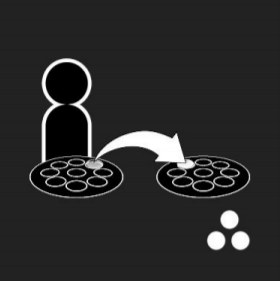
\includegraphics[scale=0.2]{black-move.png}
\end{minipage}

\begin{minipage}{0.58\textwidth}
\item O jogador representado pode mover o empregado do espaço onde está para o mesmo espaço numa mesa diferente.  \newline
\textbf{Requisito:} 5 peças iguais.
\end{minipage}
\hspace{4mm}
\begin{minipage}{0.58\textwidth}
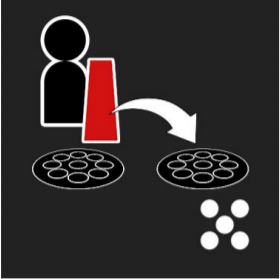
\includegraphics[scale=0.2]{black-waiter.png}
\end{minipage}

\begin{minipage}{0.58\textwidth}
\item O jogador pode rodar a mesa para uma orientação qualquer (empregado também roda). \newline
\textbf{Requisito:} 4 peças iguais.
\end{minipage}
\hspace{4mm}
\begin{minipage}{0.58\textwidth}

\includegraphics[scale=0.2]{rotate.png}
\end{minipage}

\begin{minipage}{0.58\textwidth}
\item O jogador que ativa a ação pode trocar a posição de duas mesas não conquistadas. O empregado também é movido, se presente. \newline 
\textbf{Requisito:} 4 peças iguais.
\end{minipage}
\hspace{4mm}
\begin{minipage}{0.58\textwidth}
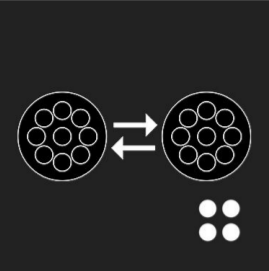
\includegraphics[scale=0.2]{swap-unclaimed.png}
\end{minipage}

\begin{minipage}{0.58\textwidth}
\item O jogador que ativa a ação pode trocar a posição de uma mesa conquistada com uma não conquistada. O empregado também é movido, se presente. \newline 
\textbf{Requisito:} 5 peças iguais.
\end{minipage}
\hspace{4mm}
\begin{minipage}{0.58\textwidth}
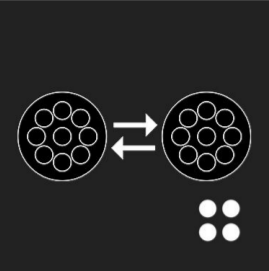
\includegraphics[scale=0.2]{swap-claimed.png}
\end{minipage}

\end{itemize}

\subsection{Conquistar uma mesa}
Quando um jogador tiver 5 peças da sua cor numa mesa, conquista essa mesa. A mesa pode continuar a ser utilizada nas jogadas, mas quando todos os espaços vazios forem preenchidos a mesa será considerada completa e qualquer jogada que levaria um jogador a ir para essa mesa será substituída, fazendo com que o jogador possa escolher um lugar qualquer vazio para colocar a sua peça.

\subsection{Fim do Jogo}
Quando um jogador conquista 5 das 9 mesas o jogo acaba imediatamente.

%%%%%%%%%%%%%%%%%%%%%%%%%%
\newpage
\section{Representação do Estado do Jogo}
A representação do estado do jogo não se poderá cingir apenas ao armazenamento do tabuleiro, dada a existência de elementos exteriores dinâmicos - as cartas especiais.

Para tal, considerou-se favorável a utilização de uma estrutura de dados adicional - uma lista que correlaciona os marcadores especiais e as mesas.

De facto, seria possível a reserva de um elemento extra na representação de cada mesa, mas por motivos de simplificação e facilidade de impressão do tabuleiro, dividiu-se em dois arrays distintos.

\subsection{Tabuleiro}
O tabuleiro é uma matriz multidimensional que preserva as 9 mesas redondas, mapeadas de forma similar ao teclado numérico de um telemóvel:

\begin{itemize}
\itemsep0em
\item A \textbf{1ª posição} da matriz corresponde à mesa \textbf{Noroeste} (NW).
\item A \textbf{2ª posição} da matriz corresponde à mesa \textbf{Norte} (N).
\item A \textbf{4ª posição} da matriz corresponde à mesa \textbf{Oeste} (O).
\item ...
\end{itemize}

A correspondência de cada posição da mesa a um ponto cardeal segue o mesmo padrão.

\subsubsection{Representação inicial do tabuleiro}
No estado inicial, todas as células estão vazias - representadas por \texttt{`x'}.

\begin{wrapfigure}{R}{0.3\textwidth}
\centering
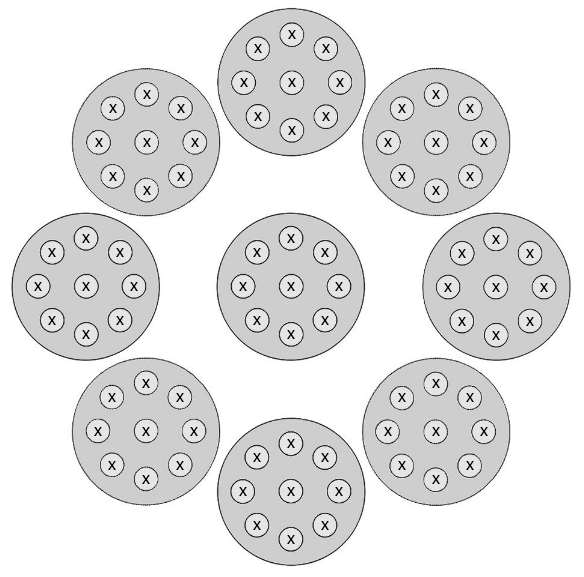
\includegraphics[width=0.18\textwidth]{board-setup-1.png}
\end{wrapfigure}

\begin{lstlisting}
  [[x, x, x, x, x, x, x, x, x],
   [x, x, x, x, x, x, x, x, x],
   [x, x, x, x, x, x, x, x, x],
   [x, x, x, x, x, x, x, x, x],
   [x, x, x, x, x, x, x, x, x],
   [x, x, x, x, x, x, x, x, x],
   [x, x, x, x, x, x, x, x, x],
   [x, x, x, x, x, x, x, x, x],
   [x, x, x, x, x, x, x, x, x]]
\end{lstlisting}

\subsubsection{Representação intermédia do tabuleiro}
No estado intermédio, surge o aparecimento de peças pretas - representadas por \texttt{`b'} - e peças verdes - representadas por \texttt{`g'}.

\begin{wrapfigure}{R}{0.3\textwidth}
\centering
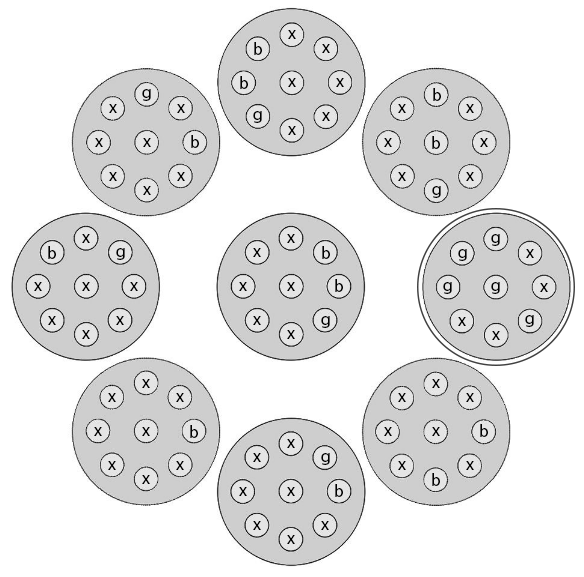
\includegraphics[width=0.18\textwidth]{board-setup-2.png}
\end{wrapfigure}

\begin{lstlisting}
  [[x, g, x, x, x, b, x, x, x],
   [b, x, x, b, x, x, g, x, x],
   [x, b, x, x, b, x, x, g, x],
   [b, x, g, x, x, x, x, x, x],
   [x, x, b, x, x, b, x, x, g],
   [g, g, x, g, g, x, x, x, g],
   [x, x, x, x, x, b, x, x, x],
   [x, x, g, x, x, b, x, x, x],
   [x, x, x, x, x, b, x, b, x]]
\end{lstlisting}

Neste estado em específico ilustrou-se uma situação de vitória de mesa por parte do jogador verde. Note-se que a mesa Este - posição nº6 da matriz - acumula um total de 5 peças verdes, pelo que a maioria nesse ponto está estabelecida.

\subsubsection{Representação final do tabuleiro}

\begin{wrapfigure}{R}{0.3\textwidth}
\centering
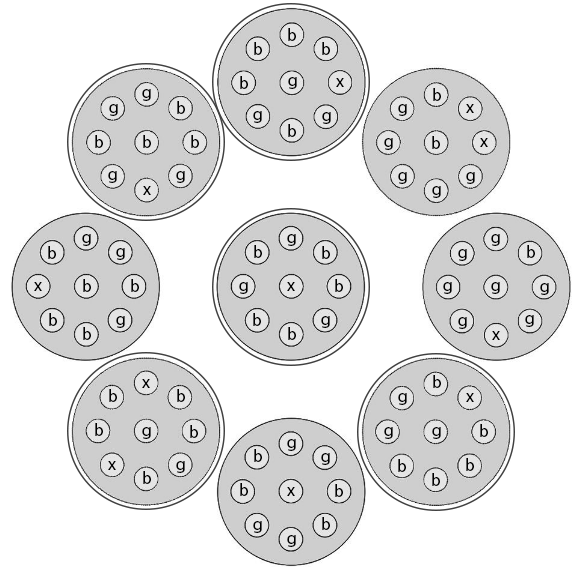
\includegraphics[width=0.18\textwidth]{board-setup-3.png}
\end{wrapfigure}


\begin{lstlisting}
  [[g, g, b, b, b, b, g, g, x],
   [b, b, b, b, g, x, g, g, b],
   [g, b, x, g, b, x, g, g, g],
   [b, g, g, x, b, b, b, b, g],
   [b, g, b, g, x, b, b, b, g],
   [g, g, b, g, g, g, g, x, g],
   [b, x, b, b, g, b, x, b, g],
   [b, g, g, b, x, b, g, g, b],
   [g, b, x, g, g, b, b, b, b]]
\end{lstlisting}

Nesta situação final, o jogador preto emerge vitorioso, tendo conquistado maioria nas cinco mesas Norte, Oeste, central, Sudoeste e Sudeste. \newline

\subsection{Marcadores especiais}

Dada a atribuição aleatória dos marcadores especiais no início do jogo e a possibilidade do jogo terminar sem todos os marcadores serem ativados, apresentar-se-á apenas uma possível disposição inicial e intermédia/final.

O mapeamento continua a executar-se do mesmo método descrito anteriormente.

\subsubsection{Representação inicial dos marcadores}
\begin{lstlisting}
  [black_move, green_move, black_waiter, green_waiter, 
   empty, rotate, rotate, swap_unclaimed, swap_claimed]
\end{lstlisting}

Neste exemplo, o marcador \textbf{black\_move} está associado à mesa Noroeste.

Note-se a repetição da carta especial \textbf{rotate}, que efetivamente possui dois exemplares, e também a utilização da etiqueta \textbf{empty} para identificar mesas sem marcadores - ora consumidos, ora não atribuídos, como no caso da mesa central. \newline

\subsubsection{Representação intermédia/final dos marcadores}
\begin{lstlisting}
  [black_move, empty, black_waiter, green_waiter, 
   empty, rotate, rotate, empty, swap_claimed]
\end{lstlisting}

Nesta etapa do jogo, os marcadores \textbf{green\_move} e \textbf{swap\_unclaimed} haverão sido consumidos, daí a sua substituição por \textbf{empty}. \newline


%%%%%%%%%%%%%%%%%%%%%%%%%%
\newpage
\section{Visualização do Tabuleiro}

A representação do tabuleiro envolve ou a sacrificação de legibilidade e acessibilidade da estrutura de dados ou uma maior complexidade na impressão do mesmo, dada a disposição circular do tabuleiro.

Optou-se por investir na facilidade de implementação da lógica e, em versões futuras, otimizar o código de impressão.

Por efeitos de simplificação, a impressão não é feita com a disposição original do jogo. Em vez disso, é utilizada uma matriz de 3x3 mesas com 3x3 posições cada uma. As posições representam, igualmente, os pontos cardeais, para facilitar o jogo.

\begin{center}
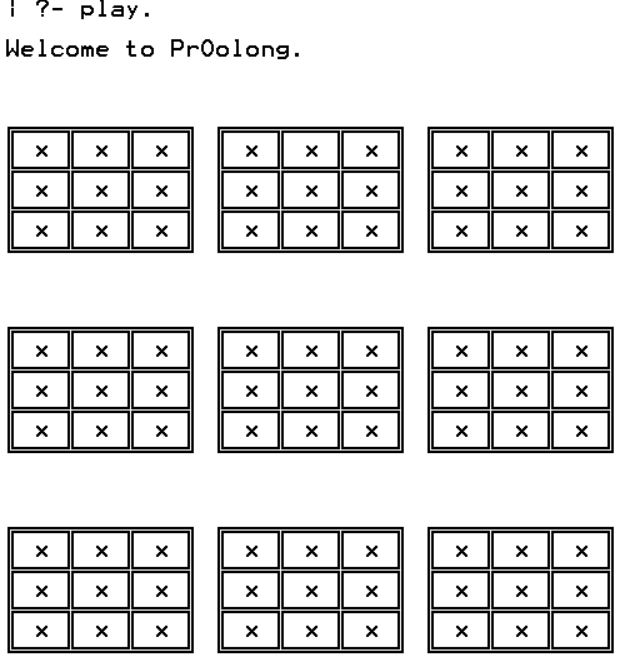
\includegraphics[scale=0.33]{tabuleiro.png}
\end{center}

Para produzir este efeito, é usado o predicado \texttt{print\_formatted\_line(X)} para desenhar as linhas horizontais em cada matriz, que separam as posições. 

Este predicado invoca chamadas \textbf{put\_code} com os códigos ASCII 185, 187, 188, 201, 204, 205 e 206. X pode levar os argumentos 0, 1, 2 ou 3 dependendo do tipo de linha a imprimir. \newline

O predicado \texttt{print\_board([H|T])} encarrega-se de, a cada iteração, separar a matriz num bloco 3x9 (3 mesas), com recurso a predicados desenvolvidos para facilitar a manipulação de listas. \texttt{trim\_head(L,N,S)} e \texttt{trim\_tail(L,N,S)} cortam \textbf{N} elementos do princípio e fim da lista \textbf{L}, respetivamente.

\begin{lstlisting}
  print_board([H|T]) :- length([H|T], Matrix_Size),
    Trim_Size is Matrix_Size - 3,
    trim_tail([H|T], Trim_Size, Block),
    print_block(Block),
    trim_head(T, 2, Remain),
    print_board(Remain).
\end{lstlisting}

\begin{lstlisting}
  trim_head(L,N,S) :- length(P,N), append(P,S,L).
  trim_tail(L,N,S) :- reverse(L,R), length(P,N), 
                      append(P,K,R), reverse(K,S). 
\end{lstlisting}

O predicado \texttt{print\_block([H|T])} imprime o bloco que lhe é passado. São usadas as funções \textbf{nth0}, \textbf{write}, \textbf{put\_code} e \textbf{print\_formatted\_line} várias vezes, permitindo desenhar a matriz linha a linha.

\begin {lstlisting}
  print_block([H|T]) :-
    print_formatted_line(0), (...)
    nth0(0, H, E1), write(E1), write(' '), (...)
    nth0(0, T, A1),
    nth0(0, A1, E4), write(E4), write(' '), (...)
\end{lstlisting}

%%%%%%%%%%%%%%%%%%%%%%%%%%
\newpage
\section{Movimentos}

Cada turno, o jogador tem acesso a dois tipos de jogadas distintos:

\begin{itemize}
\item Colocação de uma peça em Board, enviando a posição de eleição numa lista cuja cabeça \textbf{H} corresponde à mesa e a cauda \textbf{T} à cadeira.

\texttt{place\_token([H|T], Board)}

\item Caso os requerimentos para a ativação de um marcador especial se cumpram, a seleção de uma mesa \textbf{Table} do \textbf{Board} e ativação da sua habilidade é automática.

\texttt{activate\_special(Table, Board)}
\end{itemize}

Note-se, porém, que o input adicional exigido ao jogador varia consoante o marcador selecionado. \newline

Por exemplo, o marcador \textbf{rotate} permite a rotação da mesa numa direção no sentido dos ponteiros do relógio ou inverso. Para tal, um possível predicado seria \texttt{rotate\_table(Direction, Table, Board)}. 	\newline

Traduzindo, a direção \textbf{Direction} - introduzida pelo jogador - da rotação da mesa \textbf{Table}, adquirida através do predicado \textbf{activate\_special}. Estas alterações manifestam-se em \textbf{Board}. \newline

Com o desenvolvimento do projeto e avanço da lógica de jogo, mais predicados deste género serão desenvolvidos.






\end{document}
